\input{../YKY-preamble.tex}
\setmainfont[BoldFont=Alibaba_Sans_Regular.otf,ItalicFont=Alibaba_Sans_Light_Italic.otf]{Alibaba_Sans_Light.otf}
	
\usepackage[active,tightpage]{preview}		% for continuous page(s)
\renewcommand{\PreviewBorder}{0.5cm}
\renewcommand{\thempfootnote}{\arabic{mpfootnote}}

\usepackage[absolute,overlay]{textpos}		% for page number on upper left corner

\usepackage{color}
\usepackage{mathtools}
\usepackage[hyperfootnotes=false]{hyperref}

% \usepackage[backend=biber,style=numeric]{biblatex}
% \bibliography{../AGI-book}
% \renewcommand*{\bibfont}{\footnotesize}

\usetikzlibrary{shapes}
\usepackage[export]{adjustbox}				% ??
\usepackage{verbatim} % for comments
% \usepackage{newtxtext,newtxmath}	% Times New Roman font

% \numberwithin{equation}{subsection}

\newcommand{\underdash}[1]{%
	\tikz[baseline=(toUnderline.base)]{
		\node[inner sep=1pt,outer sep=10pt] (toUnderline) {#1};
		\draw[dashed] ([yshift=-0pt]toUnderline.south west) -- ([yshift=-0pt]toUnderline.south east);
	}%
}%

% Tic-Tac-Toe symbols
% \newcommand{\bO}[0]{\raisebox{-0.2em}{\textbf{O}}}
% \newcommand{\Xb}[0]{\raisebox{-0.2em}{\textbf{X}}}

%\DeclareSymbolFont{symbolsC}{U}{txsyc}{m}{n}
%\DeclareMathSymbol{\strictif}{\mathrel}{symbolsC}{74}
\DeclareSymbolFont{AMSb}{U}{msb}{m}{n}
\DeclareSymbolFontAlphabet{\mathbb}{AMSb}
% \setmathfont{Latin Modern Math}

% \newcommand{\highlight}[1]{\colorbox{pink}{$\displaystyle #1$}}

% \newcommand{\emp}[1]{{\color{violet}\textbf{#1}}}
\let\oldtextbf\textbf
\renewcommand{\textbf}[1]{\textcolor{blue}{\oldtextbf{#1}}}

\newcommand{\logic}[1]{{\color{violet}{\textit{#1}}}}
\newcommand*\smileFace{$\vcenter{\hbox{\includegraphics[scale=0.6]{../smiley.jpg}}}$}
\newcommand{\underconst}{\includegraphics[scale=0.5]{../2020/UnderConst.png}}
\newcommand{\KBsymbol}{\vcenter{\hbox{\includegraphics[scale=1]{../KB-symbol.png}}}}
\newcommand{\witness}{\scalebox{0.6}{$\blacksquare$}}
% \newcommand{\Heytingarrow}{\mathrel{-}\mathrel{\triangleright}}
% \providecommand\Heytingarrow{\relbar\joinrel\mathrel{\vcenter{\hbox{\scalebox{0.75}{$\rhd$}}}}}

\begin{document}

\begin{preview}

\cc{
\title{\vspace{-1.5cm} \bfseries\color{blue}{\Large 逻辑与深度学习的关系}}
}{
\title{\vspace{-1.5cm} \bfseries\color{blue}{\Large Comparison of Logic AI and Deep Learning}}
}

% \author{YKY} % Your name
\date{\vspace{-2cm}} % Date, can be changed to a custom date

\maketitle

\setcounter{section}{-1}

% (1) Circled page number on upper left corner
\begin{textblock*}{5cm}(2.1cm,2.3cm) % {block width} (coords) 
{\color{red}{\large \textcircled{\small 1}}}
\end{textblock*}

\begin{minipage}{\textwidth}
\setlength{\parskip}{0.4\baselineskip}

这是经典逻辑 AI 的最基本运作模式:
\begin{equation}
\vcenter{\hbox{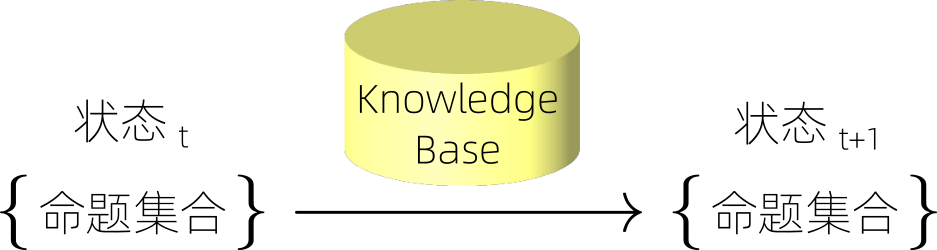
\includegraphics[scale=1]{LBAI-basic-config.png}}}
\end{equation}

它其实包含了两个算法:
\begin{itemize}
	\item \textbf{matching} (unification): \\
	逻辑 rules 是包含变量的条件命题, \\
	例如 \tab \logic{$\forall x. \mbox{是人}(x) \Rightarrow \mbox{会死}(x). $ }\\
	Unification 判定一条 rule 是否可以 apply 到某逻辑命题上,\\
	例如:\logic{是人(苏格拉底)} 可以跟上式的左边 unify. \\
	Matching 的结果是得到一推 instantiated(特例化,即不包含变量)的命题。
	
	\item \textbf{forward- or backward-chaining} (resolution): \\
	由已知事实 推导出新结论,或反过来,判断某给定的新结论是否成立。 \\
	例如:\logic{ 是人(苏格拉底) $\Rightarrow$ 会死(苏格拉底) $\;\; \wedge$ 是人(苏格拉底) } \\
	可以推出:\logic{会死(苏格拉底)}。
\end{itemize}

深度学习的特点,就是将
\begin{equation}
\mbox{状态}_t  \vdash \mbox{状态}_{t+1}
\end{equation}
的逻辑推导过程,通通纳入进去一个非常复杂的非线性函数(= 深度神经网络)里面。 这样做以后,上述的逻辑结构被
``mingled'' 在一起,以至于很难分辨了。 但也正是由于这种「大杂烩」,深度神经网络 将一套复杂的组合算法 压缩成数量不算太多的一层层的参数。 它同时可以做 learning 和 inference 这两个动作。 这种简单粗暴的方法,其实非常有效率,要超越它的速度并不容易!

我们知道(或推测)一个智能系统 应该具有 符号逻辑的结构。 这点知识可不可以用来 约束/加速 深度神经网络? 答案似乎是有可能的。 现时 state-of-the-art 处理 视觉的 CNN 和 处理文字的 BERT,它们都有内部结构,而不是 fully-connected,而且 这内部结构 对应于 被处理的资料的结构。 因此我们有理由相信,逻辑结构 可以用来约束 深度神经网络的结构,达到加速。 

\end{minipage}
\end{preview}

\begin{preview}
\begin{minipage}{\textwidth}
\setlength{\parskip}{0.4\baselineskip}

\begin{textblock*}{20cm}(2.1cm,2cm) % {block width} (coords) 
	{\color{red}{\large \textcircled{\small 2}}}
	\hspace{8cm}
	\color{blue}{\footnotesize \cc{逻辑与深度学习}{Logic and Deep Learning}}
\end{textblock*}
\vspace*{0.3cm} 

接下来我们详细一点看逻辑系统的结构:

Knowledge Base 里面有很多 rules,系统要将这些 rules 逐一 match with 系统状态 (= working memory) 里面的命题:
\begin{equation}
\vcenter{\hbox{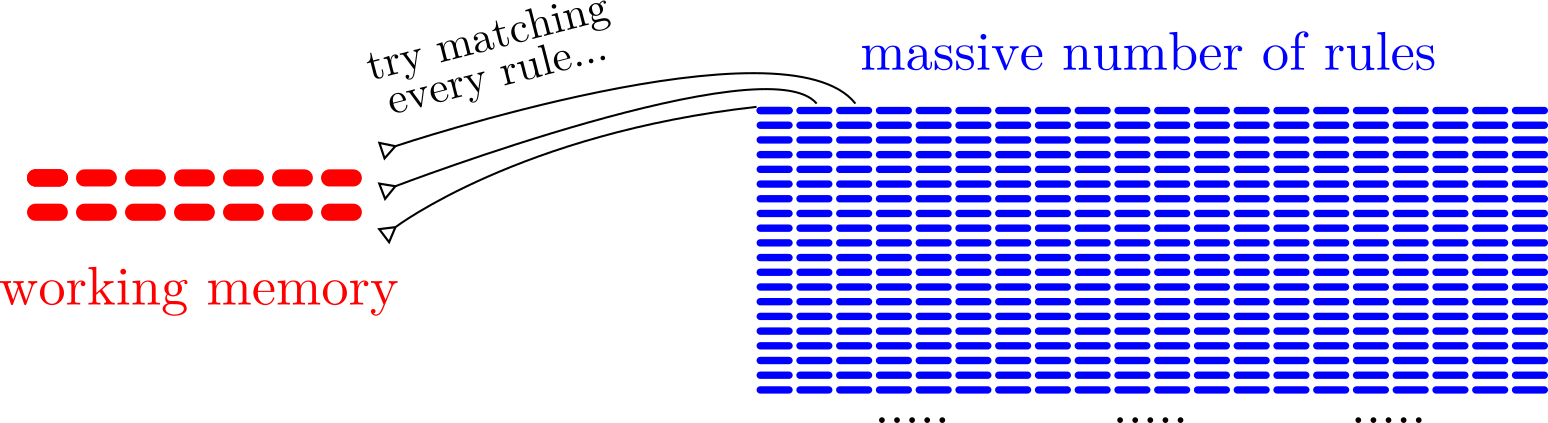
\includegraphics[scale=1]{rete-explained-1.png}}}
\end{equation}
成功 matched 的 rules 可以导出新的结论,加进 working memory 的状态 里面。

这个复杂的操作,完全被一个神经网络取代。 或者可以更抽象地说:
\begin{equation}
\vcenter{\hbox{
\includegraphics[scale=1]{some-kind-of-memory.png}}}
\end{equation}

而以 Transformer 来说,它是一种 输入元 \textbf{之间} 的记忆体(这记忆就储存在 Q, K, V 矩阵里),而它 \textbf{implicitly} 做到了 rules 的作用:
\begin{equation}
\vcenter{\hbox{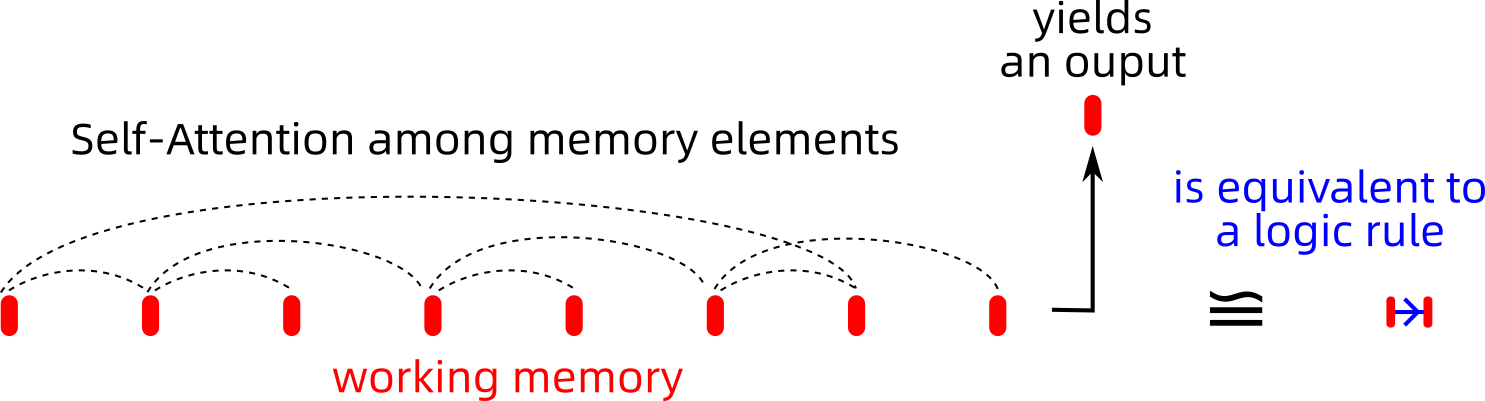
\includegraphics[scale=1]{rete-explained-3b.png}}}
\end{equation}
换句话说,Transformer 内部有 逻辑 rules 的结构。 那么很自然的问题就是,能否发掘更多 逻辑/逻辑系统 的结构? 这个问题 已部分地被 范畴逻辑 理论解决了。

那么逻辑结构 必然带来一些 代数结构,我们希望

\end{minipage}
\end{preview}

\begin{preview}
\begin{minipage}{\textwidth}
	
\setlength{\parskip}{0.4\baselineskip}
\begin{textblock*}{20cm}(2.1cm,2cm) % {block width} (coords) 
	{\color{red}{\large \textcircled{\small 3}}}
	\hspace{8cm}
	\color{blue}{\footnotesize \cc{Transformer 的逻辑解释}{Transformer as Logic}}
\end{textblock*}

\vspace*{0.3cm} 


\end{minipage}
\end{preview}

\begin{preview}
\begin{minipage}{\textwidth}

\setlength{\parskip}{0.4\baselineskip}
\begin{textblock*}{20cm}(2.1cm,2cm) % {block width} (coords) 
	{\color{red}{\large \textcircled{\small 4}}}
	\hspace{8cm}
	\color{blue}{\footnotesize \cc{Transformer 的逻辑解释}{Transformer as Logic}}
\end{textblock*}

\vspace*{0.3cm} 


\end{minipage}
\end{preview}
\end{document}
